%
% linse.tex
%
% (c) 2019 Prof Dr Andreas Müller, Hochschule Rapperswil
%
\subsection{Dünne Linse\label{mo:subsection:linse}}
Eine Linse besteht aus zwei sphärischen Flächen mit 
Krümmungsradien $R_1$ und $R_2$ (Abbildung~\ref{mo:focus}).
Die Brechungsindexverhältnisse an den beiden Flächen sind reziprok,
also $\nu_2=\nu_1^{-1}$.
Da die Linse als dünn angenommen wird, kann der Abstand der beiden Flächen
vernachlässigt werden, wir nehmen daher $x_1=x_2$ an.

Die Transformatrix des Systems wird daher durch die Matrix
\begin{align*}
T
&=
T_x
B(\nu_2, R_2)
B(\nu_1, R_1)
T_{-x_0}
\\
&=
\begin{pmatrix}
1&x\\
0&1
\end{pmatrix}
\begin{pmatrix}
1&0\\
\frac1{R_2}(\nu^{-1}-1)&\nu^{-1}
\end{pmatrix}
\begin{pmatrix}
1&0\\
\frac1{R_1}(\nu-1)&\nu
\end{pmatrix}
\begin{pmatrix}
1&-x_0\\
0&1
\end{pmatrix}
\\
&=
\begin{pmatrix}
1&x\\
0&1
\end{pmatrix}
\begin{pmatrix}
1&0\\
\frac1{R_2}(\nu^{-1}-1)+\nu^{-1}\frac{1}{R_1}(\nu-1)&1
\end{pmatrix}
\begin{pmatrix}
1&-x_0\\
0&1
\end{pmatrix}
\\
&=
\begin{pmatrix}
1&x\\
0&1
\end{pmatrix}
\begin{pmatrix}
1&0\\
\displaystyle
\biggl(\frac1{R_2}-\frac1{R_1}\biggr)(\nu^{-1}-1)
&1
\end{pmatrix}
\begin{pmatrix}
1&-x_0\\
0&1
\end{pmatrix}
\end{align*}
beschrieben.
Für eine Linse in Luft kann man $n_1=1$ setzen, dann ist $\nu=n_1/n_2$
und damit $\nu^{-1}=n_2$.
Damit ist Transfermatrix
\[
T
=
\begin{pmatrix}
1&x\\
0&1
\end{pmatrix}
\begin{pmatrix}
1&0\\
\displaystyle
\biggl(\frac1{R_2}-\frac1{R_1}\biggr)(n_2-1)
&1
\end{pmatrix}
\begin{pmatrix}
1&-x_0\\
0&1
\end{pmatrix}.
\]

\subsubsection{Brennweite}
\begin{figure}
\centering
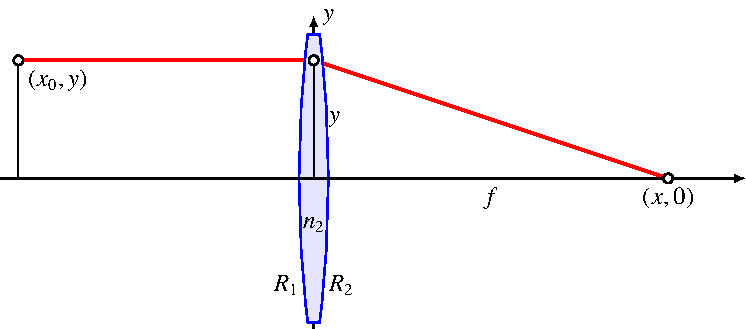
\includegraphics{applications/matrixoptik/fl.pdf}
\caption{Brennweite einer dünnen Linse
\label{mo:focus}}
\end{figure}
Die Brennweite einer Linse ist der Werte $x$, bei dem parallel zur
optischen Achse auf die Linse fallende Strahlen in einem Punkt
zusammenkommen (Abbildung~\ref{mo:focus}).
Ein Strahl parallel zur optischen Achse hat $\alpha_0=0$.
Gesucht wird also dasjenige $x$, für welches der $y$-Wert unter der
Wirkung von $T$ zu $0$ wird:
\begin{align*}
\begin{pmatrix}
0\\?
\end{pmatrix}
&=
T
\begin{pmatrix}y_0\\0\end{pmatrix}
=
\begin{pmatrix}
1&x\\
0&1
\end{pmatrix}
\begin{pmatrix}
1&0\\
\displaystyle
\biggl(\frac1{R_2}-\frac1{R_1}\biggr)(n_2-1)
&1
\end{pmatrix}
\begin{pmatrix}
1&-x_0\\
0&1
\end{pmatrix}
\begin{pmatrix}y_0\\0\end{pmatrix}
\\
&=
\begin{pmatrix}
1&x\\
0&1
\end{pmatrix}
\begin{pmatrix}
1&0\\
\displaystyle
\biggl(\frac1{R_2}-\frac1{R_1}\biggr)(n_2-1)
&1
\end{pmatrix}
\begin{pmatrix}y_0\\0\end{pmatrix}
\\
&=
\begin{pmatrix}
1&x\\
0&1
\end{pmatrix}
\begin{pmatrix}y_0
\\
\displaystyle\biggl(\frac1{R_2}-\frac1{R_1}\biggr)(n_2-1)y_0
\end{pmatrix}
\\
&=
\begin{pmatrix}
y_0 + \displaystyle x\biggl(\frac1{R_2}-\frac1{R_1}\biggr)(n_2-1)y_0
\\
?
\end{pmatrix}.
\end{align*}
Die Brennweite kann gefunden werden, indem man die Gleichung
\[
0=
y_0 + \displaystyle x\biggl(\frac1{R_2}-\frac1{R_1}\biggr)(n_2-1)y_0
\]
nach $x$ auflöst.
Man erhält
\[
x
=
\biggl(
\frac{1}{R_1}-\frac{1}{R_2}
\biggr)^{-1}
(n_2-1)^{-1}.
\]
\begin{satz}
Die Brennweite einer dünnen Linse aus einem Medium mit Brechungsindex $n$ 
mit Krümmungsradien $R_1$ und $R_2$ der Flächen ist
\[
f = \biggl(\frac{1}{R_1}-\frac{1}{R_2}\biggr)^{-1} \frac{1}{n-1}.
\]
\end{satz}

Mit diesem Ausdruck für $f$ kann die Transfermatrix etwas vereinfacht
werden.
Sie lautet
\begin{equation}
T
=
\begin{pmatrix}1&x\\0&1\end{pmatrix}
\begin{pmatrix}1&0\\-f^{-1}&1\end{pmatrix}
\begin{pmatrix}1&x_0\\0&1\end{pmatrix}
\label{om:fokusmatrix}
\end{equation}

\subsubsection{Abbildungsgleichung}
\begin{figure}
\centering
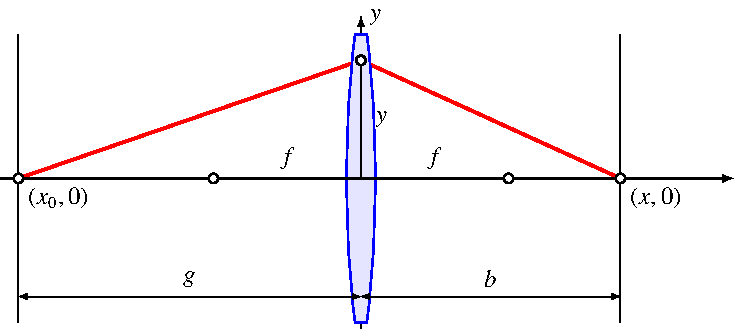
\includegraphics{applications/matrixoptik/abb.pdf}
\caption{Abbildung eines Punktes durch eine dünne Linse.
\label{mo:abb}}
\end{figure}
Wo wird das Licht, welches vom Punkt $x_0$ auf der optischen
Achse ausgeht von einer dünnen Linse fokusiert?

Diese Situation ist in Abbildung~\ref{mo:abb} dargestellt.
Wir betrachten einen Strahl, der vom Punkt $x_0$ 
auf der optischen Achse ausgeht und die Linse auf der Höhe $y$ 
trifft.
Der Winkel zur optischen Achse dieses Strahls ist $\alpha_0=y/x_0$.
Wir suchen also wieder den Punkt $x$ derart, dass der Strahl
wieder durch die optische Achse geht.
Dies bedeutet, dass
\[
\begin{pmatrix} 0\\ y/x \end{pmatrix}
=
T
\begin{pmatrix} 0\\ y/x_0 \end{pmatrix}
\]
sein muss.
Verwenden wir die Form \eqref{om:fokusmatrix} für die Transfermatrix,
erhalten wir die Bedingung
\begin{align*}
\begin{pmatrix}0\\-y/x\end{pmatrix}
&=
T
\begin{pmatrix}0\\ y/x_0\end{pmatrix}
=
\begin{pmatrix}1&x\\0&1\end{pmatrix}
\begin{pmatrix}1&0\\-f^{-1}&1\end{pmatrix}
\begin{pmatrix}1&x_0\\0&1\end{pmatrix}
\begin{pmatrix}0\\ y/x_0\end{pmatrix}
\\
&=
\begin{pmatrix}1&x\\0&1\end{pmatrix}
\begin{pmatrix}1&0\\-f^{-1}&1\end{pmatrix}
\begin{pmatrix}y\\y/x_0\end{pmatrix}
\\
&=
\begin{pmatrix}1&x\\0&1\end{pmatrix}
\begin{pmatrix}y\\ -yf^{-1}+y/x_0\end{pmatrix}
\\
&=
\begin{pmatrix} y-xyf^{-1}+xy/x_0\\ -yf^{-1}+y/x_0 \end{pmatrix}.
\end{align*}
Die erste Komponente dieser Gleichung ist
\begin{align}
0&= y-xyf^{-1}+xy/x_0.
\notag
\intertext{Dividiert man dies durch $xy$ und bringt $f^{-1}$ auf die linke
Seite findet man}
\frac{1}{f}
&=
\frac1x +\frac{1}{x_0}.
\label{om:abbildungsgleichung}
\end{align}
Die zweite Komponente stimmt automatisch überein, wenn 
\eqref{om:abbildungsgleichung} erfüllt ist.
Die Gleichung
\eqref{om:abbildungsgleichung} heisst die {\em Abbildungsgleichung}
einer Linse mit der Brennweite $f$.
Sie besagt, dass ein Objekt im Abstand $-x_0$ von einer Linse mit Brennweite
$f$ fokusiert wird im Abstand $x$ von der Linse.

\begin{satz}
Eine dünne Linse mit Brennweite $f$ bildet einen Gegenstand in der Entfernung
$g$, der {\em Gegenstandsweite}, vor der Linse in einem Punkt im Abstand $b$,
der {\em Bildweite}, hinter der Linse scharf ab, wenn die Abbildungsgleichung
\[
\frac1f = \frac1g + \frac1b
\]
gilt.
\end{satz}
